\chapter{Survey}

\label{Chapter2}

\lhead{Chapter 2. \emph{Survey}}

\section{Similar problem domains} % (fold)
\label{sec:similar_problem_domains}

Although the case in question is a specific service, the techniques in use and the limitations needing to be dealt with should apply to many kinds of applications.

When demographics are absent and identity is highly unreliable, this will unevitably lead to some highly sparse usage data and quite a bit of noise in the user modeling data.
Assuming that the usage patterns of the users actually differ, will these patterns be clearly and reliably identifiable?
Will it be possible to base an adaptive personalization system on this kind of data?
When using an anonymous system, will users welcome a personalized product, or will they regard this as breaking with their perceived concept of anonymity?

These are all questions that apply especially to appear.in, but that may also apply to many other anonymous, web-based systems.

\section{The field of user adaptation}
\label{sec:user_adaptation_survey}

This section will present an overview of the field of user adaptation. From the rather short history of the field, we move on to the conceptual frameworks and methodologies that modern adaptive systems base themselves on, before surveying the state of the art applications.

\subsection{Traditional personalization on the web}
\label{sub:traditional_web_personalization}

When the field of user adaptation meets the web, we tend to dub it either ``web personalization'' or ``adaptive hypermedia''. The terms are defined as follows:

\begin{description}
    \item[Web personalization] Any action that adapts the information or services provided by a Web site to the needs of a particular user or a set of users, taking advantage of the knowledge gained from the users' navigational behavior and individual interests, in combination with the content and the structure of the Web site~\cite{Eirinaki2003}.
    \item[Adaptive hypermedia] A hypertext or hypermedia system, with a user model, able to adapt the hypermedia using the model~\cite{Brusilovsky1996}.
\end{description}

The first definition assumes the website to be a hierarchy of content, whereas the second definition strongly relates to the concept of hypertext and hypermedia. However, large parts of the modern web have indeed shifted towards the application domain, as discussed in section~\ref{sub:the_modern_web}, where the traditional concept of a website being some kind of structured set of ``content pages'' is completely outdated. In this light, these definitions are both a bit dated.

Recent research, however, usually does not make these kinds of assumptions about the form or structure of the systems being adapted, and is mostly quite applicable for the case of modern web applications.

Thus, we will be using the terms ``user adaptation'' and ``personalization'' without relating it to the domain in which it is visible to the user, as this is quite irrelevant with a clear separation of the application and adaptational component. The evolution of this model through the 90s and into the modern internet era is elaborated on in the following sections.


\subsection{A brief history of adaptive systems}
\label{sub:adaptive_systems_history}

What is it? Other domains where it's used (marketing).

How'd it start? What use cases have been popular throughout its history? What are recent developments and key enablers?

\subsection{Conceptual framework}

\subsection{Implementation methodology}

As mentioned, there are many approaches to the task of user adaptation. Due to the constraints outlined in the previous chapters, we will be honing in on the approach termed ``web usage mining'', or sometimes ``clickstream analysis''.

Traditionally, this has entailed tracking the way users traverse a website hierarchy, looking for path patterns among them, and using this information to adapt the pages in various ways~\cite{Mobasher2000,Eirinaki2003,Montgomery2009}. While not entirely the same, this is mostly analogous to the type of adaptation problem we are solving, and the systems proposed in this earlier work solves many of the same problems that we will need to solve.

A general, high-level sketch of a typical adaptive system is outlined in figure~\ref{fig:general_adaptive_system}.

\begin{figure}[h]
  \centering
    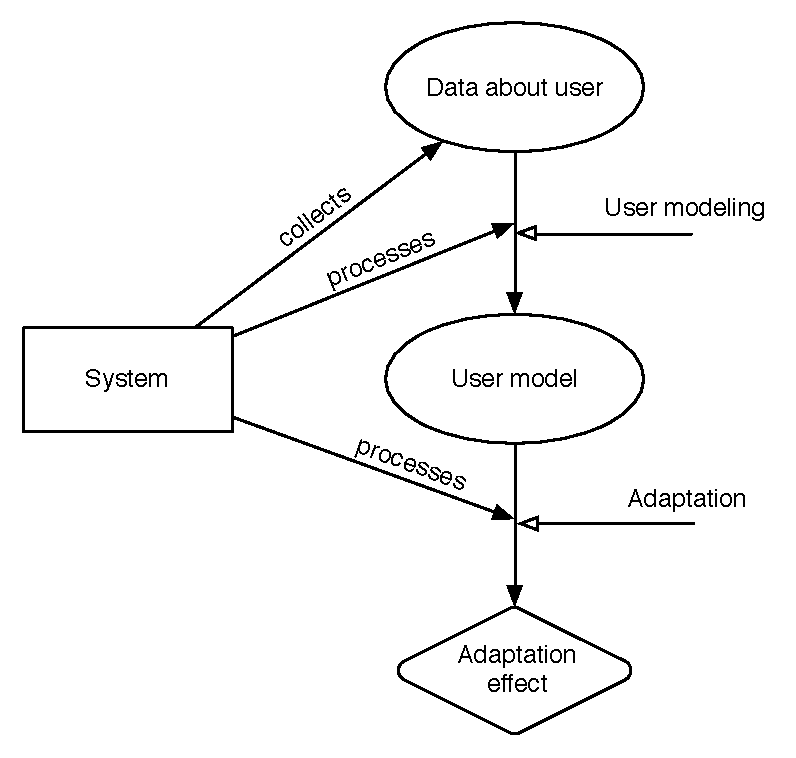
\includegraphics[width=0.8\textwidth]{Figures/adaptation-high-level}
  \caption{Caption.}
  \label{fig:general_adaptive_system}
\end{figure}

\subsection{Privacy versus personalization}
\label{survey:sec:privacy_vs_personalization}



\section{Segmentation techniques}
\label{survey:sec:segmentation_techniques}

There are several ways of

\section{A/B testing}
\label{survey:sec:ab_testing}


\section{State of the art}
\label{survey:sub:state_of_the_art}


\section{Similar research} % (fold)
\label{survey:sec:similar_applications}

The approach taken to adaptive personalization is based heavily on the work by Vrieze in ``Fundaments of Adaptive Personalization''~\cite{Vrieze}.

\subsection{Relevant literature} % (fold)
\label{survey:sec:relevant_literature}

Teltzrow and Kobsa's work on privacy-driven personalization systems provides insight into a lot of the issues surrounding the lack of demographic information in personalization~\cite{Teltzrow2004,Kobsa2007}. However, the main focus of their work seems to be that users are more willing to provide demographic information if that information is not backtracable to themselves, through pseudonymous personalization.
This matches the application in question quite poorly, as the goal is not to obtain demographics -- rather to attempt to cope without it.

\emph{@TODO} Explore and include literature on:

\begin{itemize}
  \item Clustering and segmenting users, choice of algorithms etc.
  \item Visualizing and evaluating clusters.
  \item A/B testing, multivariate testing, multi-arm bandits.
  \item Motivations for adaptive personalization. Online business models?
  \item Anonymity: do users experience personalization as an overstep?
\end{itemize}

% subsection relevant_literature (end)

% section similar_applications (end)
